\documentclass[graphics]{beamer}
\usepackage{xcolor}
\usepackage{graphicx}
\usepackage{verbatim}
\usepackage{wrapfig}
\usepackage{tabularx}
\usepackage{multirow}
\usepackage{amssymb}
\usepackage{pifont}
\usepackage{tikz}
\def\Checkmark{\tikz\fill[scale=0.2](0,.35) -- (.25,0) -- (1,.7) -- (.25,.15) -- cycle;} 

\useoutertheme{shadow}
%\usecolortheme{orchid}
\usecolortheme{seahorse}
\newcommand{\cmark}{\text{\ding{51}}}
%\newcommand*{\GtrSim}{\smallrel\gtrsim}

% math commands
\newcommand{\be}{\begin{eqnarray}}
\newcommand{\ee}{\end{eqnarray}}
\newcommand{\beq}{\begin{equation}}
\newcommand{\eeq}{\end{equation}}
\def\simless{\mathbin{\lower 3pt\hbox
      {$\rlap{\raise 5pt\hbox{$\char'074$}}\mathchar"7218$}}}
\def\simgreat{\mathbin{\lower 3pt\hbox
      {$\rlap{\raise 5pt\hbox{$\char'076$}}\mathchar"7218$}}} %> or of order

% variables

\def\toonscale{0.45}
\def\mboxy#1{\mbox{\small #1}}

\defbeamertemplate*{title page}{customized}[1][]
{
  \usebeamerfont{title}\inserttitle\par
  \usebeamerfont{subtitle}\usebeamercolor[fg]{subtitle}\insertsubtitle\par
  \bigskip
  \usebeamerfont{author}\insertauthor\par
  \usebeamerfont{institute}\insertinstitute\par
  \usebeamerfont{date}\insertdate\par
  \usebeamercolor[fg]{titlegraphic}\inserttitlegraphic
}
\begin{comment}
\AtBeginSection[]{
  \frame{
    \frametitle{Outline}
    \tableofcontents[currentsection]
  }
}
\end{comment}


\title{\textcolor{red}{Small Scale Magnetic Lenses}}
%\subtitle{}
\author[U. Pen]{{
{ 
\textcolor{green}{\small R. Main, D. Simard, D. Baker, F. Lin,
F. Kirsten, I. Yang, V. Marthi}
}, 
\textcolor{red}{\small M. van Kerkwijk, K. Vanderlinde, JP Macquart,
  U. Pen} 
}
\\[8mm] 
}
\date{\textcolor{blue}{January 10, 2017}}


\begin{document}


%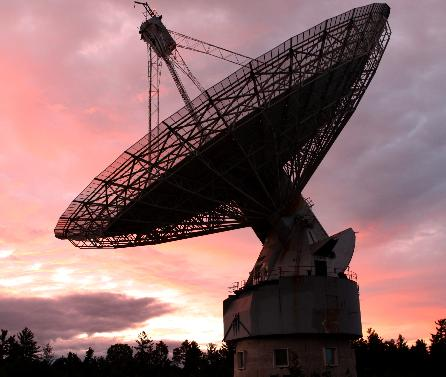
\includegraphics[width=4.4in]{Figures/IMG-7749-ARO-crop.JPG}

\frame{
\vspace{-0.5in}
\begin{center}  
%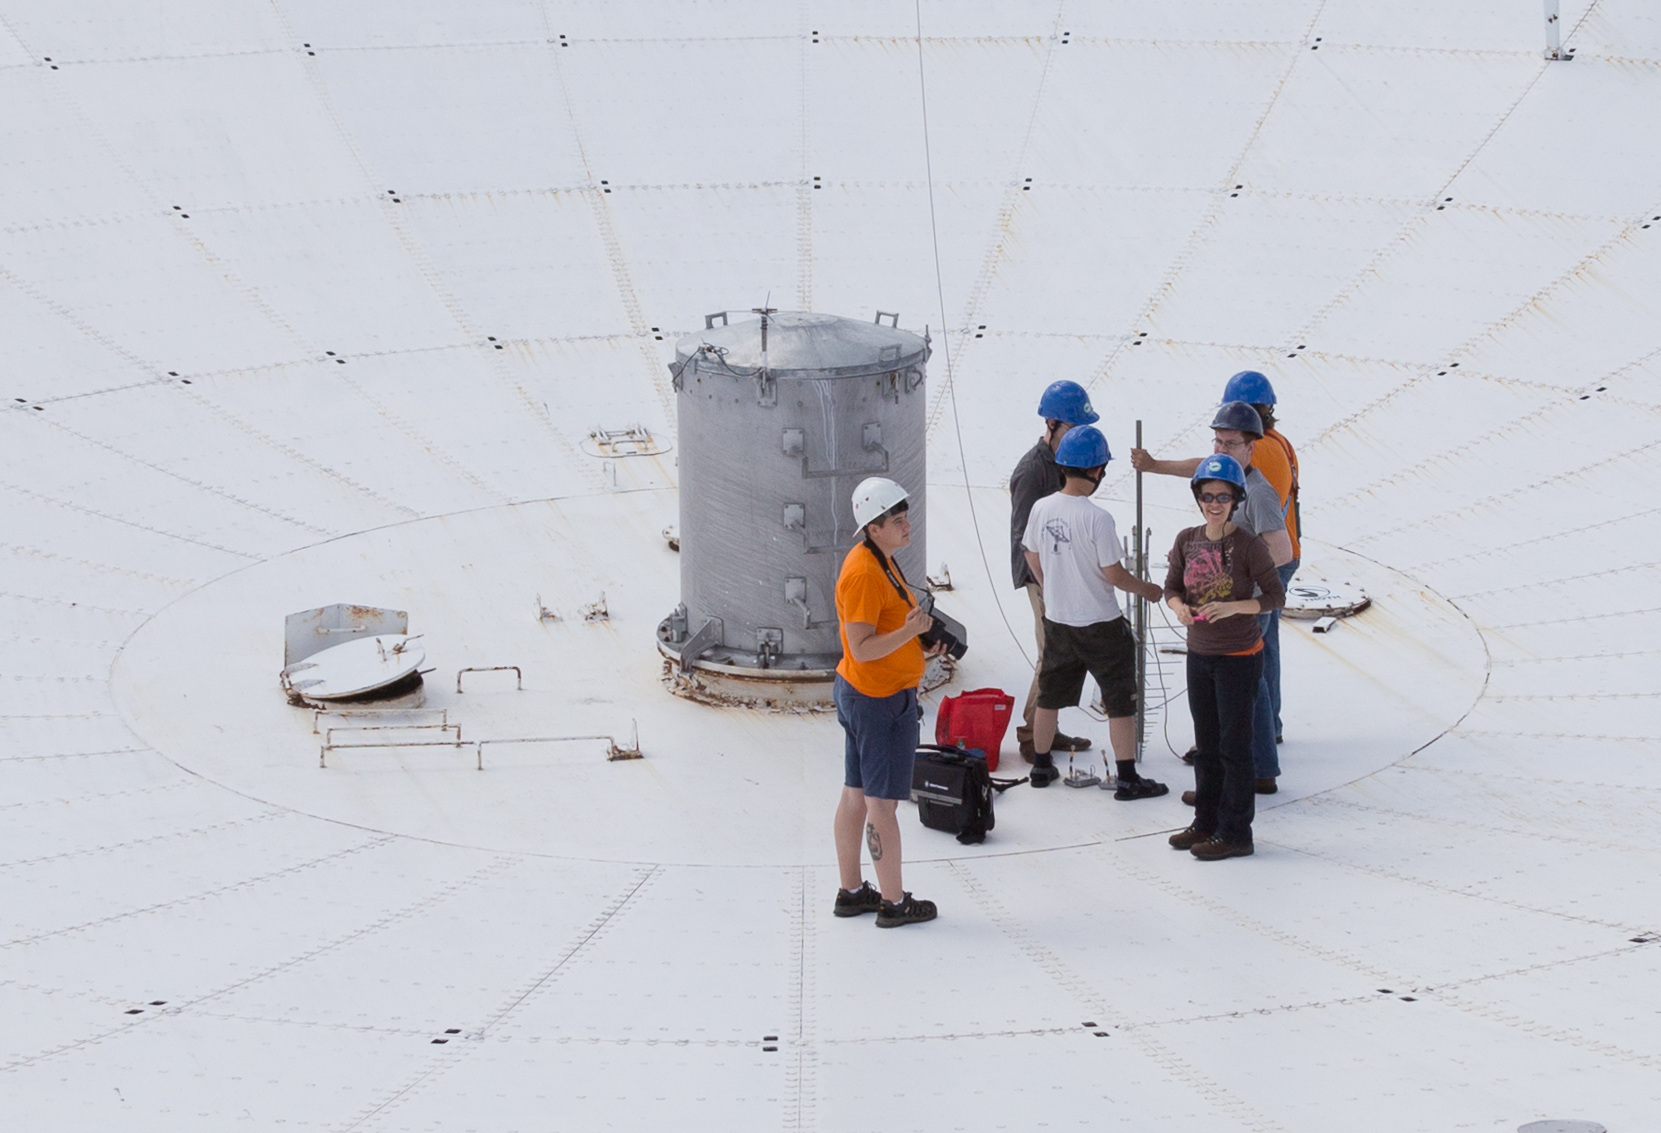
\includegraphics[width=4.4in]{Figures/IMG-0438-by-Andre-cropped.jpg}
\end{center}
\begin{picture}(320,250)
\put(-50,60){
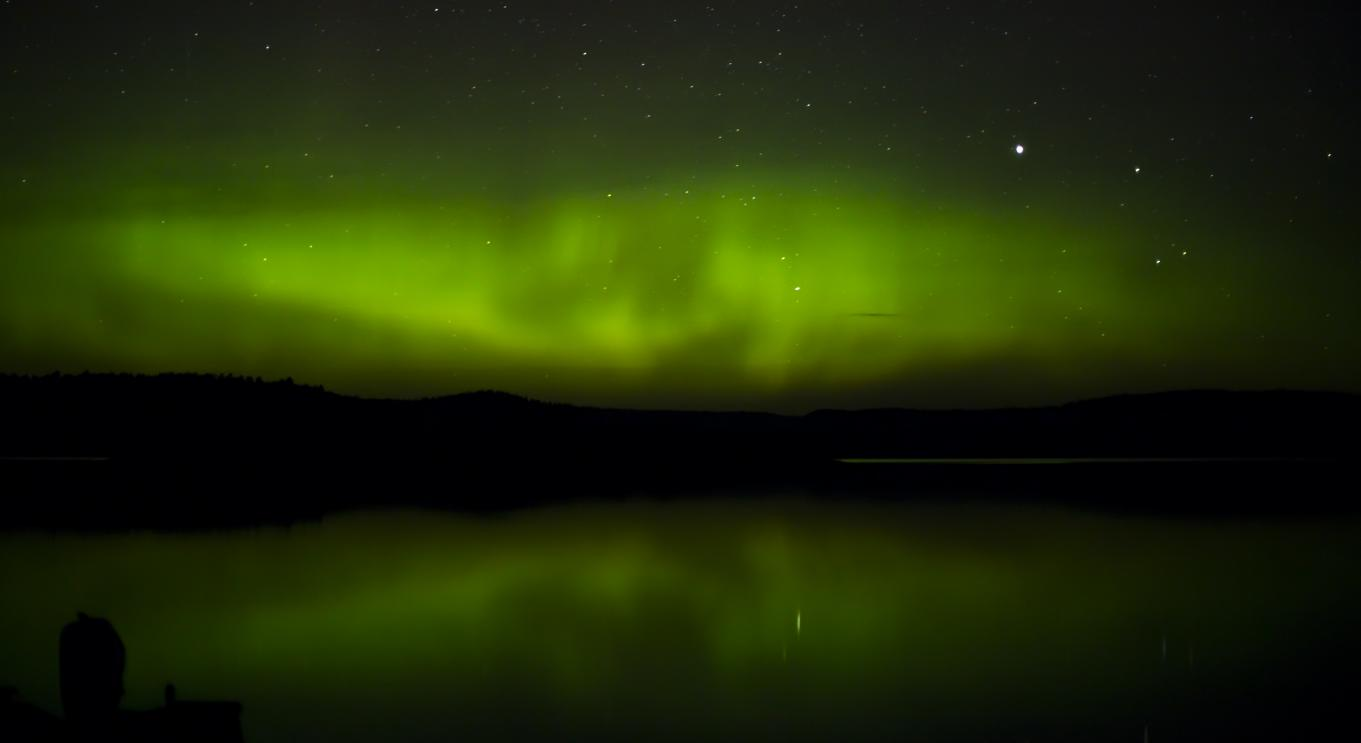
\includegraphics[width=5.5in]{Figures/traverse-aurora.jpg}}
\end{picture}
\vspace{-4in}
\\
image credit: Andre Recnik
\\
\vspace{1in}
\titlepage
}


%\section*{Introduction}
\section{Introduction}

\begin{comment}
  \subsection{Outline}

  \frame{
    \frametitle{Outline}
    \tableofcontents
  }
\end{comment}

  \frame{
    \frametitle{Overview}
    \begin{itemize}
      \item lensing: diffractive vs refractive
      \item Turbulence?
      \item magnetism
      \item Scintillometry
      \item FRBs
      \item magnetars
      \item pulsars
    \end{itemize}
    \vspace{-1in}\hspace{2in}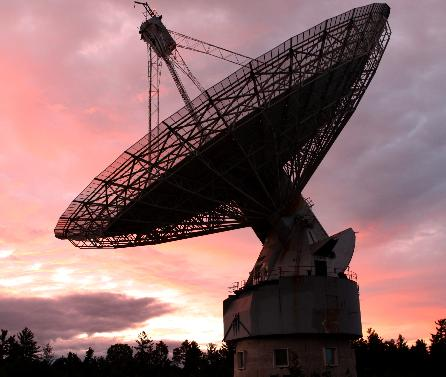
\includegraphics[width=0.5\textwidth]{Figures/IMG-7749-ARO-crop.JPG}
  }
  \frame{
    \frametitle{Scintillometry}
PSR B0834+06: 

$D_S=620$pc, 

$D_L=389/415$pc

{\tiny Brisken+2010, Liu+2016}
\begin{picture}(320,250)
\put(110,90){
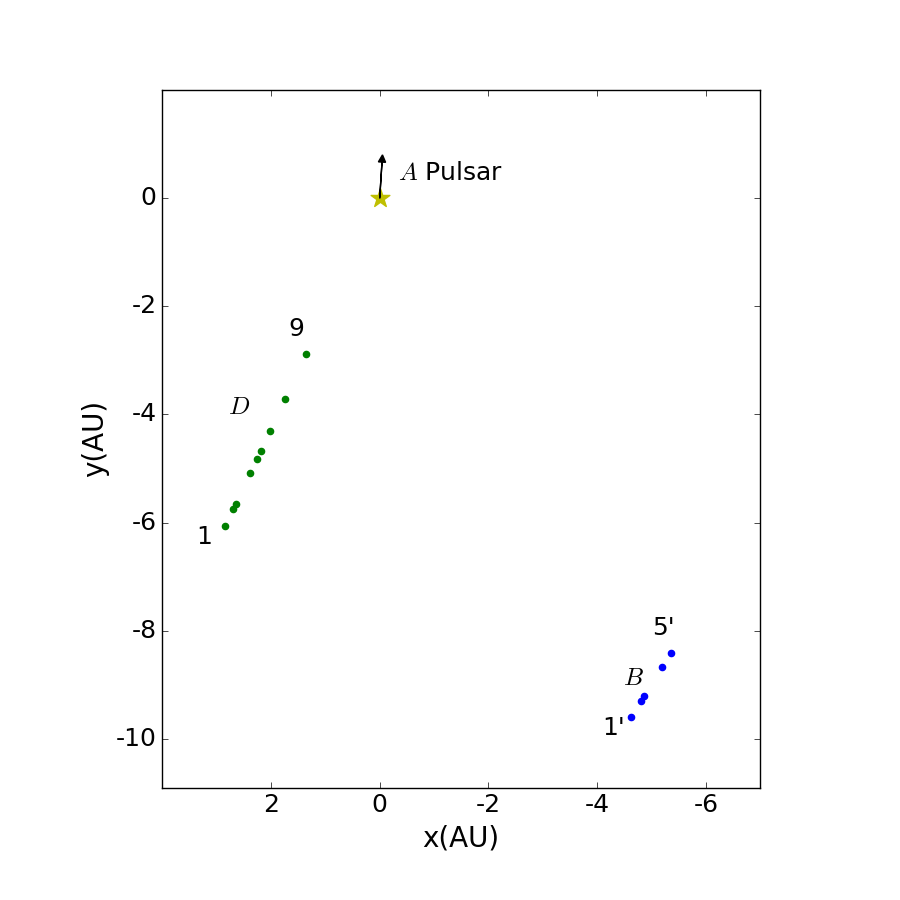
\includegraphics[width=0.7\textwidth]{Figures/Fig7_without_lines_5.png} 
}
\end{picture}
%\vspace{-4in}

  }

\frame{
    \frametitle{Lensing}
    \begin{itemize}
      \item geometric optics: refraction -- Snell's law
        $\frac{\sin\theta_1}{\sin\theta_2}=\frac{n_2}{n_1}$
      \item e.g. twinkling stars, eyeglasses
      \item multiple geometric images, that may interfere
      \item chromatic, $\Delta \theta\propto \lambda^2$
      \item wave optics --  diffraction: $\Delta \theta = \frac{\lambda}{L}$
        \item e.g. grating, hologram
        \item requires tiny scale structures
        \item misinterpreted as source of pulsar scintillation
%      \item chromatic, $\Delta \theta\propto \lambda$
    \end{itemize}
\vspace{-1.01in}
\hspace{2in}
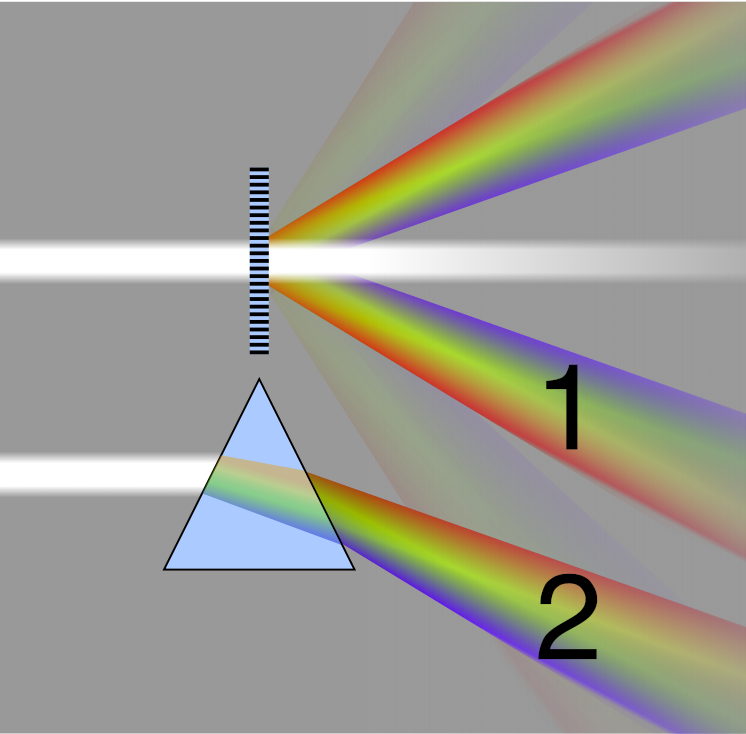
\includegraphics[width=0.3\textwidth]{Figures/prism.png}
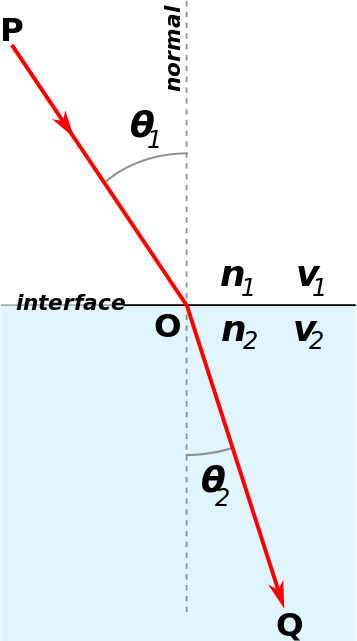
\includegraphics[width=0.3\textwidth]{Figures/Snells_law2.png}

\vspace{-0.5in}
\tiny (from wikipedia)
\vspace{0.5in}
\vspace{0.9in}
}



\section{Lensing}

\frame{
    \frametitle{Turbulence}
    \begin{itemize}
      \item observed on large scales in the ISM, outer scale $\sim 100$pc
      \item inner scale of $<1000$km proposed based on pulsar
        scintillation
      \item at odds with damping physics -- invoke undetermined plasma effects
      \item at odds with secondary spectra inverted parabolic arcs
        (Stinebring++ 2010++) and VLBI (Brisken et al 2010)
      \item intermittent, non-Gaussian, omni-predictive
      \item common misconception: pulsar scintillation is related to turbulence
    \end{itemize}

}


  \frame{
    \frametitle{Grazing incidence}
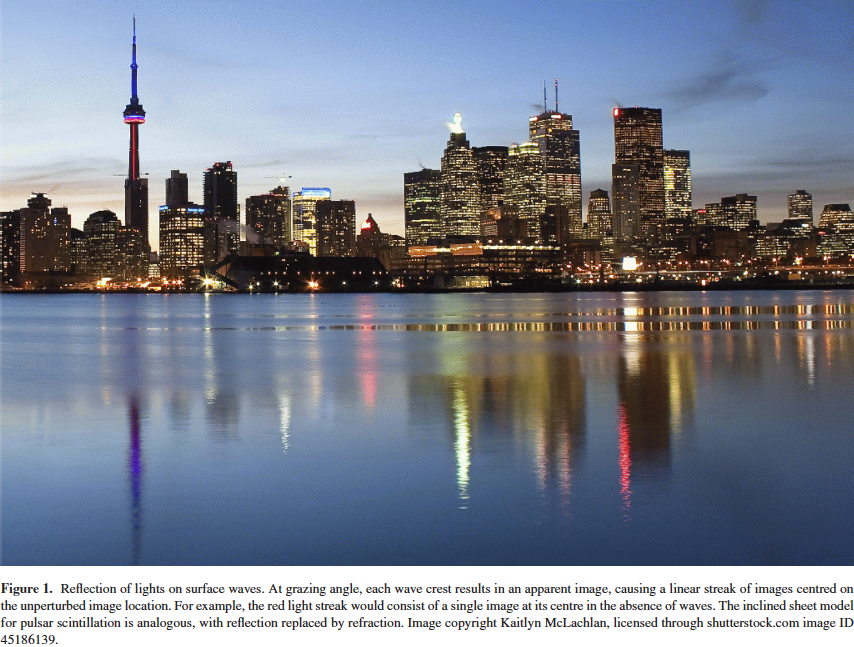
\includegraphics[width=0.9\textwidth]{Figures/toronto.png}
  }


\frame{
    \frametitle{Interference}
    \begin{itemize}
      \item Goldreich Sridhar 2006: refractive images generically
        interfere, e.g. double slit
      \item leads to scintillation scaling $\Delta \nu\propto \nu^{-4}$
      \item projected density caustics: Snell's law diverges
      \item statistics of alignment: rare alignments dominate
        lensing/scattering
      \item use ISM as giant billion km telescope!
    \end{itemize}

\tiny (from wikipedia)

\vspace{-0.5in}\hspace{2.55in}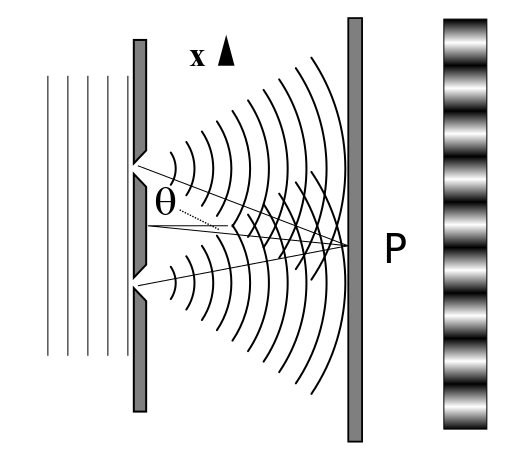
\includegraphics[width=0.4\textwidth]{Figures/Doubleslit.png}
}

\section{Magnetism}
\frame{
    \frametitle{Magnetism}
    \begin{itemize}
      \item ISM: (almost) perfect conductor (not superconductor)
      \item local lowest energy state is straight field
      \item impeded by topological entanglement (Braitwaite++ 2004++),
        Gruzinov 2009
      \item originally proposed for Ap stars and white dwarfs
    \end{itemize}
    \vspace{-0.1in}\hspace{3in}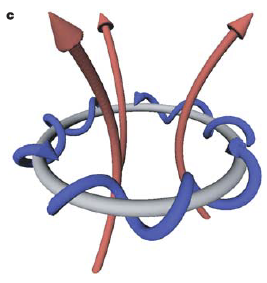
\includegraphics[width=0.3\textwidth]{Figures/braithwaite.png}
}


  \frame{
    \frametitle{Current Sheets}
    \begin{itemize}
      \item magnetic field directional change is exact solution to MHD equilibrium
      \item stability unknown, meta-stable (Sweet-Parker 1957+) or unstable (tearing
        mode, Petscheck 1964, +++)
      \item proposed as source of scattering (Goldreich-Sridhar 2006,
        Pen-Levin 2014)
    \end{itemize}
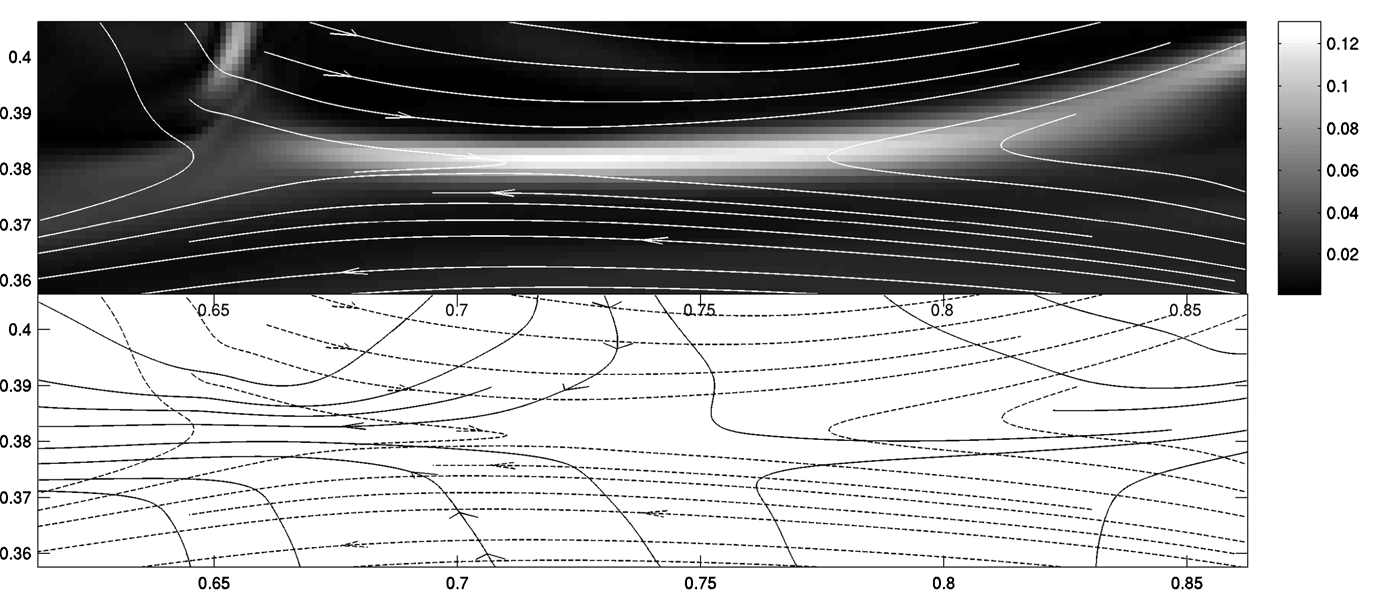
\includegraphics[width=0.9\textwidth]{Figures/reconnection.png} \tiny (Pang+2011)
  }

  \frame{
    \frametitle{Revisit}
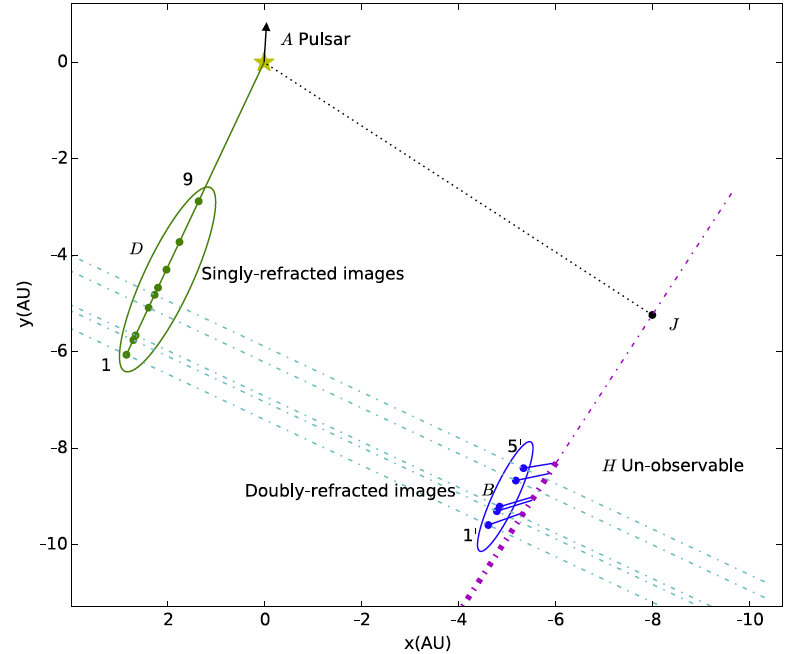
\includegraphics[width=0.8\textwidth]{Figures/liu-lens.png} \tiny
Brisken+2010, Liu+Pen 2016
  }


  \frame{
    \frametitle{Lensing}
    \begin{itemize}
      \item underdense $\longrightarrow$ convergent
      \item overdense $\longrightarrow$ divergent
      \item fold $\longrightarrow$ violate odd image theorem
      \item only one image per wave period, not 4
    \end{itemize}
\vspace{-0.75in}\hspace{3.5in}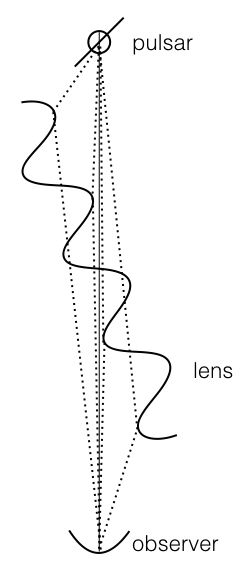
\includegraphics[width=0.25\textwidth]{Figures/convergent_geometry.jpeg}
  }
  \frame{
    \frametitle{Applications}
    \begin{itemize}
      \item cosmic telescope: picoarcsecond astrometry of magnetospheres
      \item measured 1km motion of PSR B0834+06 emission, initial results for crab
      \item potential for precision distances to pulsars, increased
        PTA sensitivity, accurate GW localization.
    \end{itemize}
%\vspace{-0.5in}\hspace{3.5in}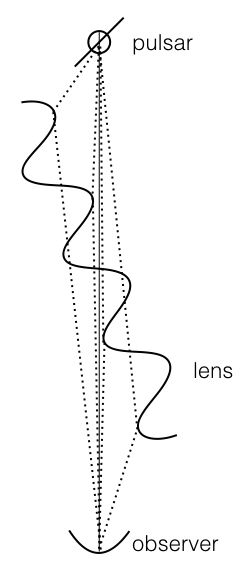
\includegraphics[width=0.15\textwidth]{Figures/convergent_geometry.jpeg}
  }
 

  \frame{
    \frametitle{FRB}
    \begin{itemize}
    \item Masui+ 2015, FRB110523: lensing of tail by milky way localizes scattering screen to host
      galaxy, rules out IGM scattering
    \item  repeating FRB: potential to discriminate AGN from nebula
    \end{itemize}
  }

  \frame{
    \frametitle{Magnetars}
    \begin{itemize}
    \item 'best bet' candidate for FRBs
    \item archetype: PSR J1745-2900
    \item hyperstrong scattering: scattering dominated at $<4$GHz.
    \item time resolved VLA/VLBA 3-D imaging: two screens, N-S screen at 3.4
      kpc, E-W at 4.4 kpc
    \end{itemize}
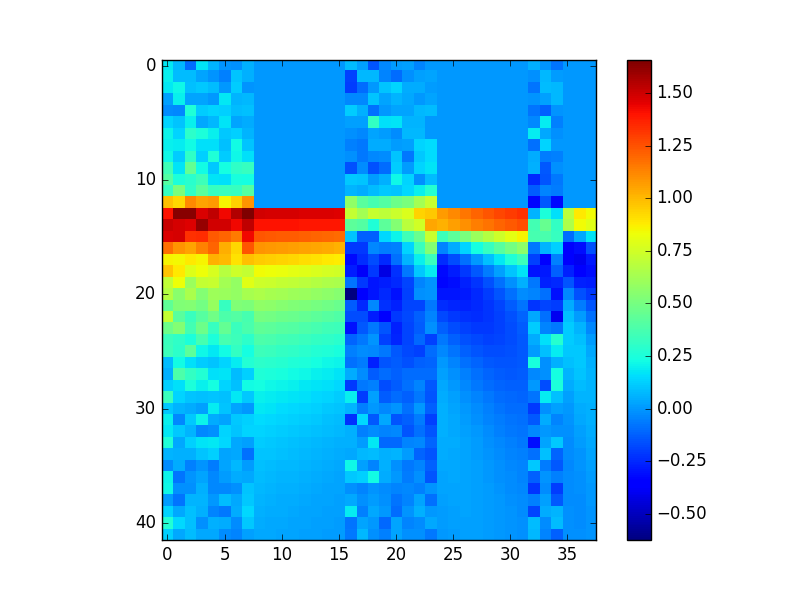
\includegraphics[width=0.5\textwidth]{Figures/fringes.png}
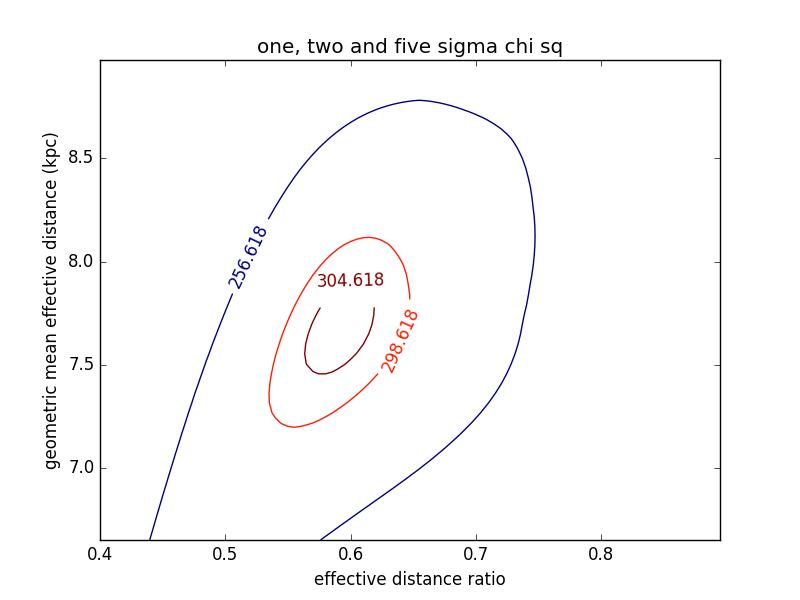
\includegraphics[width=0.5\textwidth]{Figures/analyze_search.png}
  }
  \frame{
    \frametitle{Pulsars}
    \begin{itemize}
    \item map magnetospheres: first fringes on crab with GMRT-MWA,
      DRAO-ARO, EVN, radioastron
    \item preliminary map of magnetosphere: pulse-interpulse widely
      separated, individual GP spatially resolved by nebula during
      strong scattering periods
     \item distances and inclinations to binary pulars: masses, sizes
       (inertia), distances
    \end{itemize}


\vspace{-0.3in}\hspace{1.8in} 
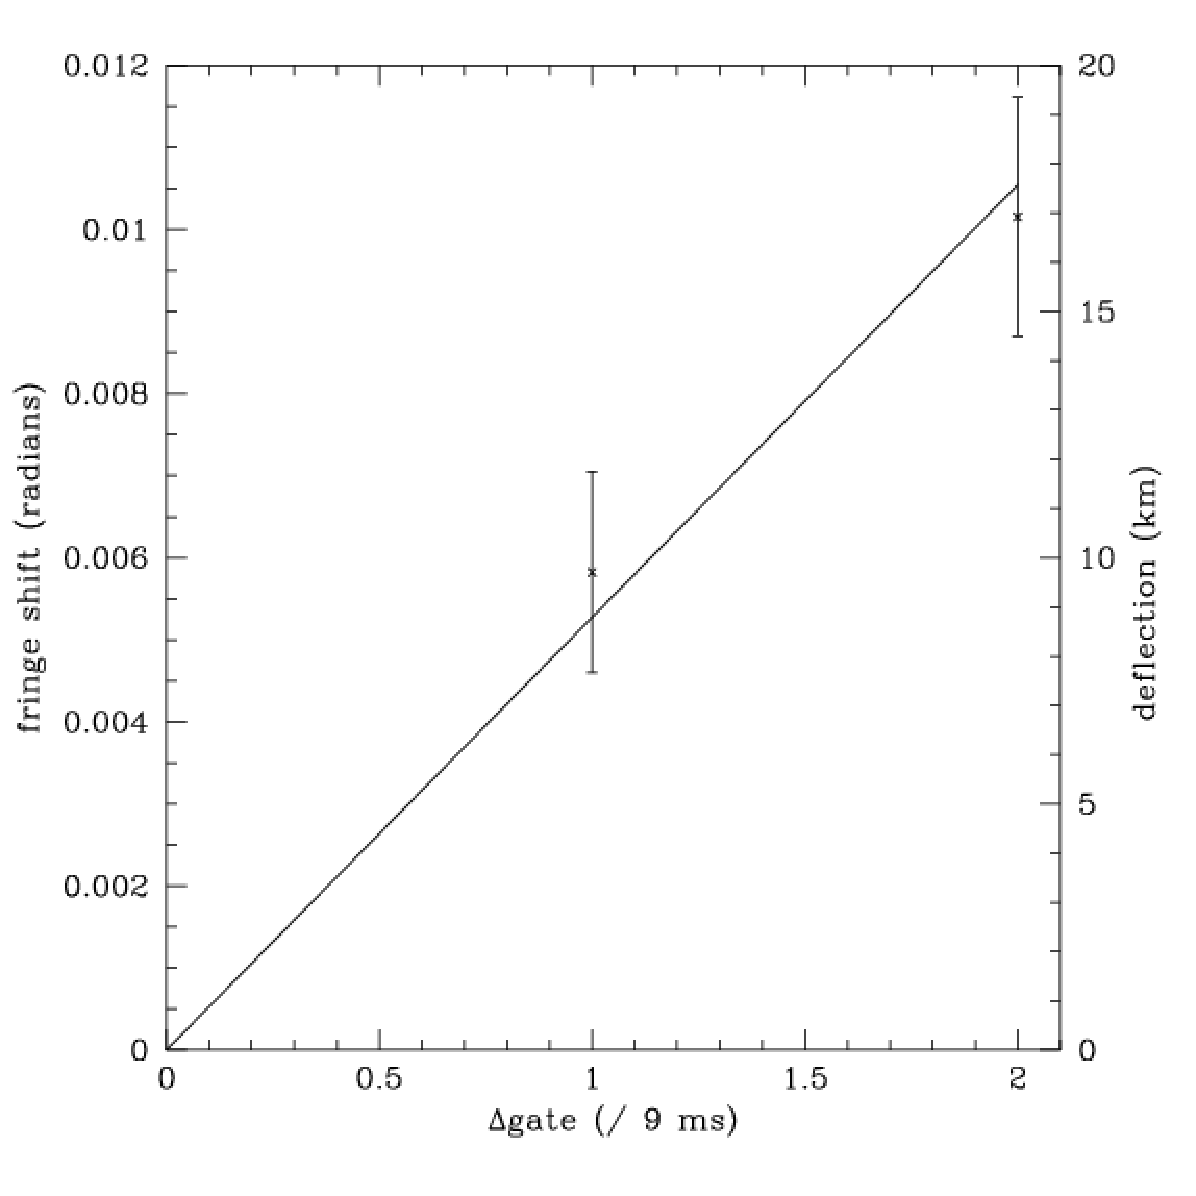
\includegraphics[width=0.4\textwidth]{Figures/allgate.pdf}
\vspace{0.5in}
\tiny Pen+ 2014

.
  }




  \frame{
    \frametitle{Discussion}
    \begin{itemize}
      \item tale of two stories
      \item turbulence: diffractive, generically not in agreement with
        data, not
        predictive, not falsifyable, information destructive
      \item Rare, thin inclined sheets: predictive, information constructive
      \item Testable with multi-epoch VLBI
    \end{itemize}
  }


  \frame{
    \frametitle{Conclusion}
    \begin{itemize}
      \item new picture of non-turbulent small scale interstellar
        plasma
        \item topologically constricted magnetic domains
      \item 1-D instead of 3-D lenses: potential to improve pulsar
        timing, mapping.
      \item potential to use scintillometry for precision pulsar
        distances, orbits, masses, improved PTA
    \end{itemize}
  }

\end{document}
